\chapter{Introduction}\label{chap:introduction}
% This introduction explains the motivation for Parallax, introduces Interaction Nets, 
% positions the work within related fields, states contributions, and outlines the dissertation.

\section{Abstract}

This dissertation introduces Parallax, a functional language compiler and runtime using interaction networks (INs) as a target to automatically parallelize sequential programs with zero programmer effort.

Parallax targets both INs for parallelism and native code for single-threaded performance, aiming for efficiency in both domains with minimal programmer intervention.

\section{Motivation}
\subsection{The Challenge of Parallel Programming}

Modern computing hardware is overwhelmingly parallel. Since the plateauing of single-core clock speed improvements around the mid-2000s, performance gains have largely arisen from increases in the number of processing cores \cite{Asanovic2006TheLandscape}. Effectively harnessing this in software, however, remains a significant challenge.

Manual parallel programming is difficult, costly, and error-prone, requiring explicit synchronization and careful management of subtle bugs like race conditions and deadlocks \cite{Lee2006TheProblem}.

Due to this complexity, hardware often remains underutilized \cite{Berzal2013}. There is a clear need for tools that automatically parallelize high-level code, easing the burden on developers.

\subsection{The Intrinsic Parallelism of Interaction Nets}

\textbf{Interaction networks (interaction nets or INs)}, introduced by Yves Lafont in 1990, offer a compelling alternative model of computation derived from the proof structures of linear logic \cite{lafont1990interactionnets}. INs provide a graphical formalism of computation based on graph rewriting, where computation proceeds through local transformations governed by simple, predefined rules. 

\newpage

INs consist of typed \textbf{agents} (nodes) with one \textbf{principal port} and \(n\) \textbf{auxiliary ports} (arity \(n\)), connected by \textbf{wires} (edges). Unconnected ports are known as \textbf{free ports}.

\begin{figure}[h]
    \centering
    \begin{tikzpicture}
        \inetmulticell(alpha){$\alpha$}{1}{7}{0,0}[U] % Pointing Up
        \inetwirefree(alpha.pal 1) % Free wire for principal port
        \node[above=2ex] at ($(alpha.pal 1)!0.5!(alpha.above pal 1)$) {principal port};
        \inetwirefree(alpha.pax 1) % Free wire for aux port 1
        \node[below left=0ex and 0.5ex] at ($(alpha.pax 1)!0.5!(alpha.above pax 1)$) {auxiliary port 1};
        \node at (alpha.above pax 4) {$\ldots$}; % Unshifted dots
        \inetwirefree(alpha.pax 7) % Free wire for aux port 7
        \node[below right=0ex and 0.5ex] at ($(alpha.pax 7)!0.5!(alpha.above pax 7)$) {auxiliary port n};
    \end{tikzpicture}
    \caption{An interaction net agent with arity $n$}
    \label{fig:intro_agent}
\end{figure}
% TODO: Diagram of agent with principal and auxiliary ports and labels

INs are defined by an \textbf{interaction system}, which consists of:

\begin{itemize}
    \item A (possibly infinite) alphabet of \textbf{types} and their respective arities.
    \item A set of \textbf{interaction rules}, which specify the possible local transformations of the network between every possible pair of nodes.
\end{itemize}

Computation proceeds by rewriting \textbf{active pairs} (connections between principal ports) using predefined \textbf{interaction rules}, replacing the pair with a new network fragment and rewiring auxiliary ports \cite{lafont1990interactionnets}.

\begin{figure}[h!]
    \centering
    \begin{tikzpicture}[scale=0.8, transform shape, wirestyle/.style={draw, line width=0.15ex}] % Use thinner lines
        % LHS
        \inetcell[arity=2](c1){C}{0,0}[R]; % Pointing Right
        \inetcell[arity=2](c2){C}{1.5,0}[L]; % Pointing Left, moved slightly
        \inetshortwire(c1.pal 1)(c2.pal 1); % Shorter wire for principal ports
        
        \inetwirefree(c1.pax 1);
        \node[above left=0.5ex and 0.5ex] at (c1.pax 1) {a}; % Label below
        \inetwirefree(c1.pax 2);
        \node[below left=0.5ex and 0.5ex] at (c1.pax 2) {b}; % Label below
        
        \inetwirefree(c2.pax 1);
        \node[below right=0.5ex and 0.5ex] at (c2.pax 1) {c}; % Label below
        \inetwirefree(c2.pax 2);
        \node[above right=0.5ex and 0.5ex] at (c2.pax 2) {d}; % Label below
        
        % Arrow
        \coordinate (mid) at (2.75, 0); % Increased distance
        \draw [->, thick] (mid) -- ++(1.25, 0);

        % RHS - Using coordinates and draw for plain lines
        \coordinate (a_coord) at (5.0, 0.5);
        \coordinate (c_coord) at (6.5, 0.5);
        \coordinate (b_coord) at (5.0, -0.5);
        \coordinate (d_coord) at (6.5, -0.5);

        \node[left=0.5ex] at (a_coord) {a};
        \node[right=0.5ex] at (c_coord) {c};
        \draw[wirestyle] (a_coord) -- (c_coord); % Connect a to c with plain line

        \node[left=0.5ex] at (b_coord) {b};
        \node[right=0.5ex] at (d_coord) {d};
        \draw[wirestyle] (b_coord) -- (d_coord); % Connect b to d with plain line

    \end{tikzpicture}
    \caption{Example Reduction Rule: C $\sim$ C $\rightarrow$ (a $\leftrightarrow$ c), (b $\leftrightarrow$ d)}
    \label{fig:intro_annihilation_rule}
\end{figure}

\subsubsection{Example: Church Numerals and Addition}

To illustrate the reduction process, consider the representation of natural numbers using Church numerals within interaction combinators. We define two basic agents:
\begin{itemize}
    \item \textbf{Zero (Z):} An agent with arity 0 (no auxiliary ports). Represents the number 0.
    \item \textbf{Successor (S):} An agent with arity 1. Represents the successor function (adding 1).
\end{itemize}
A number $n$ is represented by applying $S$ $n$ times to $Z$. For example, the number 2 is represented as the net $S(S(Z))$.

\begin{figure}[h!]
    \centering
    \begin{tikzpicture}[scale=0.8, transform shape]
        % Number 2 Representation
        \inetcell[arity=1](s1){Z}{0,0}[R];
        \inetcell[arity=1](s2){S}{$(s1.pax)+(1.5,0)$}[R]; % Use calc relative to s1's port
        \inetcell[arity=0](z){S}{$(s2.pax)+(1.5,0)$}[R]; % Use calc relative to s2's port
        \inetwire(s1.pal)(s2.pax);
        \inetwire(s2.pal)(z.pax);
        \inetwirefree(z.pal);
    \end{tikzpicture}
    \caption{Interaction Net Representation of Church Numeral 2}
    \label{fig:intro_church_two}
\end{figure}

Now, let's introduce an agent for addition:
\begin{itemize}
    \item \textbf{Add (+):} An agent with arity 2. The two operands are connected to the left auxiliary port and the principal port; while the result is available from the right auxiliary port.
\end{itemize}

The key interaction rules for addition are:

\begin{figure}[h!]
    \centering
    % Rule: + ~ S
    \begin{tikzpicture}[scale=0.7, transform shape, node distance=0.5cm and 1.5cm, wirestyle/.style={draw, line width=0.15ex}] % Adjusted node distance
        % LHS: + ~ S on second aux port
        \inetcell[arity=2](add1){+}{0,0}[R];
        \inetcell[arity=0](s1){Z}{1.5,0}[L];
        \inetwire(add1.pal 1)(s1.pal 1); % Active Pair
        \inetwirefree(add1.pax 1);
        \inetwirefree(add1.pax 2);

        % Arrow
        \draw [->, thick] (2.5, 0) -- ++(1, 0); % Adjusted arrow start

        \node at (4.5, 0) {\Huge $\supset$};

        \inetcell[arity=2](add2){+}{10,0}[R];
        \inetcell[arity=1](s2){S}{11.5,0}[L];
        \inetwire(add2.pal 1)(s2.pal 1); % Active Pair
        \inetwirefree(add2.pax 1);
        \inetwirefree(add2.pax 2);
        \inetwirefree(s2.pax);

        \draw [->, thick] (12.8, 0) -- ++(1, 0); % Adjusted arrow start

        \inetcell[arity=2](add3){+}{16.5,0}[R];
        \inetcell[arity=0](s3){S}{15.2,-0.5}[L];
        \inetwire(add3.pax 2)(s3.pax); % Active Pair
        \inetwirefree(add3.pax 1);
        \inetwirefree(add3.pal 1);
        \inetwirefree(s3.pal);
    \end{tikzpicture}
    \caption{Key Interaction Rules for Addition: $+ \sim S$ and $+ \sim Z$}
    \label{fig:intro_add_rules}
\end{figure}

Consider reducing $1 + 2$, represented as connecting the principal port of a `+` agent to the numeral $1$ ($S(Z)$), its first auxiliary port to the numeral $2$ ($S(S(Z))$), and leaving the second auxiliary port as the result output. The reduction proceeds step-by-step solely through local rule applications (Figure \ref{fig:intro_reduce_add_one_two}).

\begin{figure}[h!]
    \centering
    % Step 1: Initial State: +(S(Z), S(S(Z)))
    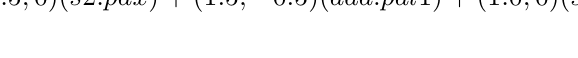
\begin{tikzpicture}[scale=0.6, transform shape] % pal is principal, pax is auxiliary
        \inetcell[arity=0](z){Z}{0,0}[R];
        \inetcell[arity=1](s){S}{$(z.pax)+(1.5,0)$}[R];
        \inetcell[arity=1](s2){S}{$(s.pax)+(1.5,0)$}[R];
        \inetcell[arity=2](add){+}{$(s2.pax)+(1.5,-0.5)$}[R];
        \inetcell[arity=1](s3){S}{$(add.pal 1)+(1.0,0)$}[L];
        \inetcell[arity=0](z3){Z}{$(s3.pax)+(1.0,0)$}[L];
        \inetwire(z.pal)(s.pax);
        \inetwire(s.pal)(s2.pax);
        \inetwire(s2.pal)(add.pax 1);
        \inetwirefree(add.pax 2);
        \inetwire(add.pal)(s3.pal)
        \inetwire(s3.pax)(z3.pal)

        \draw [->, thick] (8, -0.5) -- ++(1, 0);

        \inetcell[arity=0](z){Z}{11,0}[R];
        \inetcell[arity=1](s){S}{$(z.pax)+(1.5,0)$}[R];
        \inetcell[arity=1](s2){S}{$(s.pax)+(1.5,0)$}[R];
        \inetcell[arity=2](add){+}{$(s2.pax)+(1.5,-0.5)$}[R];
        \inetcell[arity=1](s3){S}{$(s2.pax)+(0.5,-1)$}[L];
        \inetcell[arity=0](z3){Z}{$(add.pal)+(1.0,0)$}[L];
        \inetwire(z.pal)(s.pax);
        \inetwire(s.pal)(s2.pax);
        \inetwire(s2.pal)(add.pax 1);
        \inetwirefree(s3.pal);
        \inetwire(add.pal)(z3.pal)
        \inetwire(s3.pax)(add.pax 2)

        \draw [->, thick] (18, -0.5) -- ++(1, 0);

        \inetcell[arity=0](z){Z}{21,0}[R];
        \inetcell[arity=1](s){S}{$(z.pax)+(1.5,0)$}[R];
        \inetcell[arity=1](s2){S}{$(s.pax)+(1.5,0)$}[R];
        \inetcell[arity=1](s3){S}{$(s2.pax)+(1.5,0)$}[R];
        \inetwire(z.pal)(s.pax);
        \inetwire(s.pal)(s2.pax);
        \inetwire(s2.pal)(s3.pax);
        \inetwirefree(s3.pal);
        
        
    \end{tikzpicture}
    \caption{Reduction Sequence: Adding $1 + 2$ using Church Numerals}
    \label{fig:intro_reduce_add_one_two}
\end{figure}

After these reductions, the network stabilizes into the Church numeral for 3 ($S(S(S(Z)))$) connected to the result port and the computation is complete.

\subsubsection{Properties}

Interaction nets are attractive as a compilation target due to these two fundamental properties:
\begin{enumerate}
    \item \textbf{Locality:} Reductions are strictly local, affecting only the interacting agents and their immediate connections.
    \item \textbf{Strong Confluence:} The final result is independent of reduction order of available active pairs, guaranteeing determinism \cite{mazza}.
\end{enumerate}

Together, locality and confluence allow for the concurrent reduction of active pairs, enabling automatic parallelization.


Theoretically, INs offer an elegant foundation for implementing optimal reduction strategies for functional languages like the lambda calculus \cite{mazza}. However, despite this theoretical appeal, realizing efficient practical implementations on conventional hardware has been challenging. Issues often arise from the overhead associated with managing the graph structure dynamically, the potential inefficiency of representing basic operations through combinators, and effective memory management during reduction \cite{Pinto2014InteractionNetsReview}.


\section{The Research Landscape}
\subsection{Interaction Network Programming Languages}

Two recent dedicated IN languages/runtimes are notable:

\subsubsection{Bend}

\texttt{Bend} \cite{BendGithub} is a high-level language designed specifically for the \textbf{Higher-order Virtual Machine (HVM)}. HVM is a massively parallel runtime for interaction combinators \cite{Lafont1995InteractionCombinators}, implemented in Rust with C and CUDA backends. \texttt{Bend} adopts a Python-inspired, functional syntax, enforcing purity and immutability for automatic parallelization. Key features include static typing (with restricted numerics), ADTs, pattern matching, and specialized `fold`/`bend` operations for consuming or generating recursive data structures. \texttt{Bend}'s philosophy relies on HVM to automatically exploit IN parallelism, aiming to make multi-core/GPU power accessible via a high-level style.

However, where Bend falls short is in its single-threaded performance. According to 
their own benchmarks \cite{BendGithub}, Bend is vastly outperformed by equivalent single-threaded programs written in traditional compiled languages (like \texttt{C via gcc}). It attempts to represent almost everything within the interaction net model, even when the overhead of this representation far outweighs the limited parallelism gains. Furthermore, Bend lacks significant optimizations in its compilation pipeline, potentially leaving substantial performance improvements unexplored.

\texttt{Bend} served as the primary inspiration for Parallax.

\subsubsection{Vine}

`Vine` \cite{VineGithub} is an experimental, Rust-inspired language exploring INs purely for CPU parallelism via its own runtime, the \textbf{Ivy Virtual Machine (IVM)}. \texttt{Vine}'s design explores functional/imperative interoperability, concepts like borrowing for memory management, and unique \textbf{inverse operators} (\texttt{\textasciitilde{}}) leveraging INs' bidirectional data flow. It represents another direction in harnessing INs, distinct from Bend's focus.


\subsection{Other Approaches to Automatic Parallelization}

The challenge of automatically parallelizing sequential code has been tackled using various techniques over several decades. Traditional \textbf{compiler-based methods} analyze sequential code (particularly loops in languages like \texttt{Fortran} and \texttt{C/C++}) using \textbf{data dependency analysis} to identify independent computations \cite{KennedyAllen2001OptimizingCompilers}. These compilers employ sophisticated \textbf{loop transformations} — such as privatization, reduction recognition, and interchange — to restructure code and eliminate dependencies. They often generate parallel code using explicit directive systems like \texttt{OpenMP} \cite{OpenMPARBP2018OpenMPSpecification}. The effectiveness of purely static analysis, however, is frequently limited by ambiguous pointer aliasing and complex memory access patterns inherent in the languages they often target, such as \texttt{C/C++} \cite{Allen1983DependenceAnalysis}.

To overcome static limitations, \textbf{speculative parallelization} techniques have been developed for hardware and software. Techniques like \textbf{Thread-Level Speculation} optimistically execute code sections in parallel. They rely on runtime mechanisms to detect and recover from any dependence violations, although this can incur potential overhead \cite{Rauchwerger1995RunTime}. More formal approaches, such as the \textbf{polyhedral model}, provide a powerful algebraic framework for analyzing and transforming loop nests with regular (affine) access patterns. This enables sophisticated optimizations for specific domains like scientific computing \cite{Bondhugula2008AutomaticDistributedMemory}.

Language design also plays a crucial role. Certain features inherently facilitate or simplify the expression and potential for automatic parallelization compared to imperative languages with complex state and aliasing. Examples include \texttt{Fortran}'s array operations; the purity of functional programming languages (e.g., \texttt{Haskell}), which makes dependencies explicit \cite{Hammond1996ParallelFunctional} and offers libraries like \texttt{Control.Concurrent} for explicit concurrency and \texttt{Control.Parallel} for semi-explicit parallelism; \textbf{Rust}'s ownership and borrowing system, which enables safe data parallelism through libraries like \textbf{Rayon} \cite{Rayon}; and the integrated parallelism and locality constructs of \textbf{Partitioned Global Address Space (PGAS) languages} (e.g., \texttt{Chapel}, \texttt{X10}) \cite{Yelick2007ProductivityParallel}.

More recently, \textbf{AI and Machine Learning} approaches have emerged. These methods use models trained on vast codebases to identify parallelization opportunities and generate parallel constructs (e.g., \texttt{OpenMP} pragmas). They can potentially surpass the limitations of purely analytical methods in some cases \cite{OMPar}. Additionally, \textbf{binary rewriting} offers a path to parallelize legacy executables when source code is unavailable, though this is challenged by the lack of high-level information \cite{Amaral2006AutomaticBinary}.


\section{Parallax: Bridging the Gap}

Throughout the research landscape, it's apparent that there currently exists no solution that is simultaneously highly performant on conventional hardware and requires zero programmer effort for parallelization. Existing interaction net languages sacrifice single-threaded performance, while traditional parallelization techniques are either more limited in scope or demand (at least some) manual effort/expertise.

This dissertation introduces Parallax, which aims to bridge this gap. Parallax is a novel programming language and runtime system designed to explore the viability of interaction nets as a foundation for efficient, automatically parallel computation of code written in a familiar functional style, without compromising single-threaded speed. Parallax is guided by several core design principles aimed at addressing these key problems:

Firstly, achieving \textbf{zero programmer effort} is paramount. Parallax aims to let developers write standard sequential code, with the runtime system handling all concurrency implicitly and automatically. There should be no need for explicit parallel programming constructs or annotations from the user.

Secondly, Parallax provides a \textbf{familiar syntax and semantics}, designed to look and feel like a typical functional programming language, focusing on expressiveness and type safety. This aims to lower the adoption barrier compared to existing IN languages, which often lack the expressiveness and type safety of mainstream functional languages and may require workarounds for model limitations (e.g., restricted numeric types in Bend and Vine).

Thirdly, \textbf{efficient reduction} is critical. The Parallax runtime must execute the generated interaction nets performantly in single-threaded scenarios while also scaling effectively across multiple cores. This necessitates addressing the inherent overheads associated with interaction net execution (like graph management) while maximizing the potential speedup from parallel reduction.

\section{Dissertation Outline}
This dissertation details the design, implementation, and evaluation of the Parallax system. 
\begin{itemize}
    \item \textbf{Chapter 2 (Preparation):} Covers goal refinement, requirements, design decisions, background research, and starting point.
    \item \textbf{Chapter 3 (Implementation):} Details the implementation of the compiler pipeline and parallel runtime system.
    \item \textbf{Chapter 4 (Evaluation):} Presents evaluation methodology, results (memory, scaling), and analysis.
    \item \textbf{Chapter 5 (Conclusions):} Summarizes contributions, lessons learned, and future work.
\end{itemize}
Appendices contain supplementary material, followed by the original project proposal.